\documentclass[xcolor={x11names,svgnames}]{beamer}

%TODO : gettimeofday

%\usepackage[]{babel}
\usepackage[T1]{fontenc}
\usepackage{cellspace}

\usepackage{amsmath}
\usepackage{amsfonts}
\usepackage{tikz}
\usepackage{xspace}
\usepackage[normalem]{ulem}
\usepackage{minted}
%\usepackage{fancybox}

%\usepackage{eurosym}
%\usepackage{marvosym}
%\usepackage{pifont}
\usepackage{xcolor}

\newcommand{\bigO}[1]{\ensuremath{\mathcal{O}\left( #1 \right)} }

\DeclareMathOperator*{\argmax}{arg\,max}

\newcommand{\red}{\alert}
\newcommand{\green}{\color{LimeGreen}}
\newcommand{\blue}{\color{cyan}}

%\usetikzlibrary{patterns}
%\usetikzlibrary{snakes}
%\usetikzlibrary{arrows}
%\usetikzlibrary{backgrounds}
%\usetikzlibrary{shapes}
%\usetikzlibrary{shadows}
%\usetikzlibrary{calc}
%\usetikzlibrary{decorations}
%\usetikzlibrary{decorations.pathreplacing}
%\usetikzlibrary{decorations.shapes}
%\usetikzlibrary{decorations.markings}
%\usetikzlibrary{positioning}
\usetikzlibrary {graphs, quotes}
\usetikzlibrary{graphdrawing}
\usegdlibrary{trees, layered}

\definecolor{amethyst}{rgb}{0.6, 0.4, 0.8}
\definecolor{cyan}{rgb}{0,0.6796875,1}

\usecolortheme{rose}
\setbeamertemplate{footline}{}
\setbeamertemplate{navigation symbols}{}

\usepackage{fontspec}
\setsansfont{PalatinoSansLTPro}[
   Path = /home/charles/charles_work/fonts/PalatinoSans/, 
   Extension      = .otf,
   UprightFont    = *-Regular,
   BoldFont= *-Bold ,
   ItalicFont = *-Italic,
   BoldItalicFont = *-BoldIta
]

\author[C.~Bouillaguet]{Charles Bouillaguet \newline
  {\small (\texttt{charles.bouillaguet@lip6.fr})}}

\title{Cours X : understanding code performance}
\date{2022-XX-XXXX}

\begin{document}

\begin{frame}[label=title]
  \titlepage
\end{frame}

%%%%%%%%%%%%%%%%%%%%%%%%%%%%%%%%%%%%%%%%%%%%%%%%%%%%%%

\begin{frame}
  \frametitle{Famous Quote}

  {\Huge \textbf{Premature optimization} \\ is the root of all evil

  \bigskip
  
  --- Donald Knuth }

\bigskip

  \begin{block}{Meaning}
    \begin{itemize}
    \item Optimization takes (programmer) time
    \item Use your time efficiently
    \item Optimization usually makes code more complex
      \begin{itemize}
      \item Harder to read/debug/maintain/upgrade
      \end{itemize}
    \item Should be done \textbf{only} when necessary
    \end{itemize}
  \end{block}
\end{frame}

%%%%%%%%%%%%%%%%%%%%%%%%%%%%%%%%%%%%%%%%%%%%%%%%%%%%%%%%%

\begin{frame}
  \begin{block}{Rule of thumb}
    \begin{itemize}
    \item 95\% of the running time...
    \item ... usually concentrated in 5\% of code statements
      \begin{itemize}
      \item E.g. inner loops, specific function, etc.
      \end{itemize}
    \item[$\leadsto$] Need to identify them
    \end{itemize}
  \end{block}
  
  \begin{alertblock}{Need}
    \begin{itemize}
    \item We need tools to \textbf{observe} code behavior
    \item \textbf{Where} does it spend most of its time?      
    \end{itemize}
  \end{alertblock}

  \begin{exampleblock}{Key idea}
    \begin{itemize}
    \item \textbf{do not} optimize code representing 0.001\% of the time
    \item Common rookie mistake
    \end{itemize}
  \end{exampleblock}

\end{frame}

%%%%%%%%%%%%%%%%%%%%%%%%%%%%%%%%%%%%%%%%%%%%%%%%%%%%%%%%%

\begin{frame}
  \frametitle{Where Does my Code Spend Its Time?}
  
  \begin{block}{Two methods}
    \begin{enumerate}
    \item Sampling
    \item Instrumentation
    \end{enumerate}
  \end{block}

  \begin{exampleblock}{Illustration / Case Study}
    \begin{itemize}
    \item Colleague from the \emph{Institut de minéralogie, de physique des
        matériaux et de cosmochimie} (Sorbonne University) 

    \item Least square fitting of model to experimental data points

    \item \textbf{Function} $f : \mathbb{R}^{n} \rightarrow \mathbb{R}^{m}$
      \begin{itemize}
      \item $f$ is computed by X million lines of ugly Fortran code
      \item $n = 1000$ (parameters to choose)
      \item $m = 10^7$ (data points to fit)
      \end{itemize}

    \item \textbf{Goal}: find $x$ that minimizes $\|f(x)\|_2$
    \item Use \texttt{MINPACK} library from 1978 --- \red{takes forever}. Why?
  \end{itemize}
    
  \end{exampleblock}
  
\end{frame}

%%%%%%%%%%%%%%%%%%%%%%%%%%%%%%%%%%%%%%%%%%%%%%%%%%%%%%%%%

\begin{frame}
  \frametitle{Sampling}

  \begin{columns}
    \begin{column}{5cm}
  \begin{block}{Main Idea}
    \begin{itemize}
    \item Just \textbf{run} the code
    \item \textbf{Interrupt it} regularly
      \begin{itemize}
      \item E.g. 1kHz
      \end{itemize}
    \item Store the \textbf{instruction pointer} (``sample'')
    \item Resume
    \end{itemize}    
  \end{block}

  \begin{exampleblock}{Afterwards}
    \begin{itemize}
    \item Look \textbf{where} it was interrupted
    \item Instruction often executed $\leadsto$ more samples
    \end{itemize}
  \end{exampleblock}
  
\end{column}
\begin{column}{6cm}
  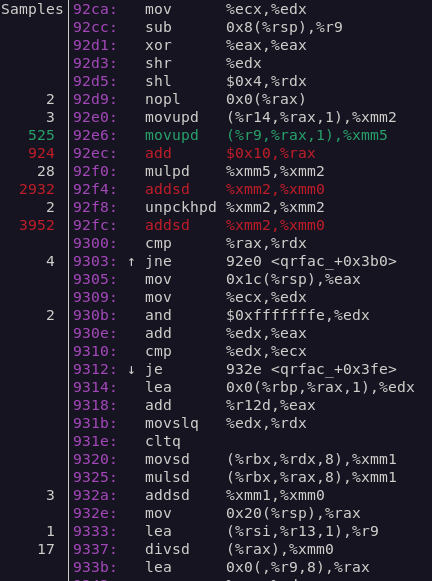
\includegraphics[width=6cm]{perf.png}
\end{column}
\end{columns}
\end{frame}

%%%%%%%%%%%%%%%%%%%%%%%%%%%%%%%%%%%%%%%%%%%%%%%%%%%%%%%%%

\begin{frame}
  \frametitle{Case Study}

  \noindent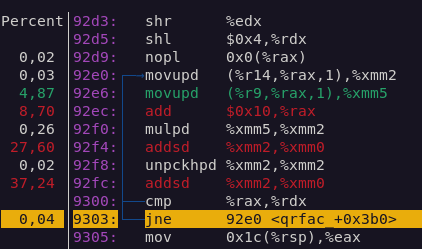
\includegraphics[width=7cm]{perf2.png}

  \begin{alertblock}{Pinpointing the Hot Spot}
    \begin{itemize}
    \item Loop of 9 CPU instructions
    \item $\approx 80\%$ of the total running time 
    \end{itemize}
  \end{alertblock}
  
  \begin{block}{Good, but...}
    \begin{itemize}
    \item Where is instruction \texttt{0x92fc} in my code? {\tiny hint: \texttt{qrfac}}
    \end{itemize}
  \end{block}
\end{frame}

%%%%%%%%%%%%%%%%%%%%%%%%%%%%%%%%%%%%%%%%%%%%%%%%%%%%%%%%%

\begin{frame}[fragile]
  \frametitle{Making Sense of Code Addresses}

  Where is instruction \texttt{0x92fc} in my code?

  \begin{exampleblock}{Good News}
    \begin{itemize}
    \item The \textbf{debugging symbols} exist to answer this question
    \item Enable debugging symbols: \texttt{gcc [...] -g [...]}
      \begin{itemize}
      \item Makes executable slightly larger...
      \end{itemize}
    \item Map between \textbf{instructions} and \textbf{source file/line}
      \begin{itemize}
      \item Sometimes not obvious with compiler optimizations
      \item May reorder code, permute loops, etc. 
      \end{itemize}
    \item Exploited by many tools: \texttt{gdb}, \texttt{valgrind}, ...
    \end{itemize}
  \end{exampleblock}

  \begin{block}{Simple tool: \texttt{addr2line}}
    \begin{verbatim}
    $ addr2line -e ./speed_lmdif1 0x92fc
    minpack/qrfac.c:134 (discriminator 3)
\end{verbatim}
    Let's look at \texttt{minpack/qrfac.c}, line 134
  \end{block}  
\end{frame}

%%%%%%%%%%%%%%%%%%%%%%%%%%%%%%%%%%%%%%%%%%%%%%%%%%%%%%%%%

\begin{frame}[fragile]
  \frametitle{Actually looking at the code}

  \begin{minted}[linenos,firstnumber=127]{C}
void qrfac_(...)
{
    for (int j = 1; j <= n; ++j) {
        // ...     
        for (int k = j + 1; k <= n; ++k) {
            double sum = 0;
            for (int i = j; i <= m; ++i)
/* !!! */       sum += a[i + j * m] * a[i + k * m];
            double temp = sum / a[j + j * m];
            for (int i = j; i <= m; ++i)
                a[i + k * m] -= temp * a[i + j * m];
            // ...
        }
        // ...  
    }
}
\end{minted}
\end{frame}

%%%%%%%%%%%%%%%%%%%%%%%%%%%%%%%%%%%%%%%%%%%%%%%%%%%%%%%

\begin{frame}
  \frametitle{Sampling --- Summary}

  \begin{block}{(Relative) Ease of Use}
    \begin{itemize}
    \item Commercial programs (Intel VTune, ...)
    \item Under linux: \texttt{perf}
      \begin{itemize}
      \item \texttt{\$ perf record ./program}
      \item \texttt{\$ perf report} 
      \end{itemize}
      
    \end{itemize}
  \end{block}

  \begin{exampleblock}{Advantages}
    \begin{itemize}
    \item Runs at $\approx$ 100\% native speed
    \item Quite precise
    \item Can measure other things than time
    \end{itemize}
  \end{exampleblock}

  
  \begin{alertblock}{Problems}
    \begin{itemize}
    \item Usually requires \textbf{administrator} privileges
    \item And/or cooperation from the operating system
    \end{itemize}
  \end{alertblock}
  
\end{frame}

%%%%%%%%%%%%%%%%%%%%%%%%%%%%%%%%%%%%%%%%%%%%%%%%%%%%%%%

\begin{frame}[fragile]
  \frametitle{Instrumentation}
  
  \begin{columns}
    \begin{column}{5cm}
  \begin{block}{Main Idea}
    \begin{itemize}
    \item \textbf{Modify} the code
      \begin{itemize}
      \item Add measurements
      \end{itemize}
    \item Run \textbf{instrumented} code
    \end{itemize}    
  \end{block}

  \begin{exampleblock}{Afterwards}
    \begin{itemize}
    \item Look at the data collected by the instrumentation
    \end{itemize}
  \end{exampleblock}
  
\end{column}
\begin{column}{6cm}
  \begin{minted}[fontsize=\scriptsize]{C}
double start = wtime();
double qrfac_time = 0;
int qrfac_calls = 0;
// ...
double qrfac_start = wtime();
qrfac(...);
qrfac_time += wtime() - qrfac_start;
qrfac_calls += 1;
// ...
double total = wtime() - start;
printf("Running time: %.1fs\n", total);
printf("%d calls to qrfac (%.1fs)\n",
    qrfac_calls, qrfac_time);
exit(0);
  \end{minted}
\end{column}
\end{columns}

\bigskip

\begin{alertblock}{[Manual | Automatic] instrumentation}
  \begin{itemize}
  \item Manual: if you know what you're looking for
    \begin{itemize}
    \item Or if you want your program to print performance results
    \end{itemize}
  \item Automatic: more heavyweight, simpler
  \end{itemize}
\end{alertblock}
\end{frame}

%%%%%%%%%%%%%%%%%%%%%%%%%%%%%%%%%%%%%%%%%%%%%%%%%%%%%%%%%%%%%

\begin{frame}
  \frametitle{Instrumentation: Goals}

  \begin{block}{What data do we obtain in the end?}
    \begin{itemize}
    \item A \textbf{Profile}
      \begin{itemize}
      \item Short summary of performance results
      \item Typically per-function
      \item Eventually call-graph informations
        \begin{itemize}
        \item ``Function A takes 95\% of the time, ...''
        \item ``...but only when it is called by function B''
        \end{itemize}
      \end{itemize}
      
    \item A \textbf{Trace}
      \begin{itemize}
      \item Log of timestamped ``events''
      \item Visual view of performance problems
      \item Very powerful, more complex to use
      \end{itemize}
    \end{itemize}
  \end{block}

  Can build a profile from a trace, but not the other way around
\end{frame}

%%%%%%%%%%%%%%%%%%%%%%%%%%%%%%%%%%%%%%%%%%%%%%%%%%%%%%%%%%%%

\begin{frame}
  \frametitle{Instrumentation: the GNU Profiler}
  \framesubtitle{Easy and Always Available}

  \begin{block}{Usage}
    \begin{itemize}
    \item Compile \textbf{and} link with: \texttt{gcc [...] -pg [...]}
      \begin{itemize}
      \item Automatic instrumentation
      \end{itemize}
    \item Run program
    \item[$\leadsto$] \texttt{gmon.out}
    \item \texttt{\$ gprof ./program}
    \end{itemize}
\end{block}
\end{frame}

%%%%%%%%%%%%%%%%%%%%%%%%%%%%%%%%%%%%%%%%%%%%%%%%%%%%%%%%%%%

\begin{frame}[fragile]
  \frametitle{GNU Profiler: Result}

  \begin{block}{Flat profile}
  \scriptsize
\begin{verbatim}
  %   cumulative   self              self     total           
 time   seconds   seconds    calls   s/call   s/call  name    
 97.91    408.82   408.82       59     6.93     6.95  qrfac_
  0.91    412.63     3.81        1     3.81     3.81  qrsolv_
  0.48    414.64     2.01    69139     0.00     0.00  ssqfcn
  0.41    416.35     1.71   207520     0.00     0.00  enorm_
  0.17    417.05     0.70        6     0.12    69.59  lmdif_
  0.11    417.49     0.44       59     0.01     0.04  fdjac2_
  0.02    417.56     0.07       61     0.00     0.06  lmpar_
  0.00    417.56     0.00    69133     0.00     0.00  fcn
  0.00    417.56     0.00       14     0.00     0.00  wtime
  0.00    417.56     0.00        6     0.00    69.59  do_test
  0.00    417.56     0.00        6     0.00     0.00  initpt
  0.00    417.56     0.00        6     0.00    69.59  lmdif1_
\end{verbatim}
\end{block}

\begin{itemize}
\item We learn that 98\% of the time is spent in \texttt{qrfac}
\item Called 59 times, $\approx 6.9$s per call
\end{itemize}
\end{frame}

%%%%%%%%%%%%%%%%%%%%%%%%%%%%%%%%%%%%%%%%%%%%%%%%%%%%%%%%%%%%

\begin{frame}[fragile=singleslide]
%  \frametitle{GNU Profiler: Result}

  \begin{block}{Call Graph}
  \tiny
\begin{verbatim}
index % time    self  children    called     name
...
-----------------------------------------------
                0.70  416.86       6/6           lmdif1_ [3]
[4]    100.0    0.70  416.86       6         lmdif_ [4]
              408.82    1.14      59/59          qrfac_ [5]
                0.07    3.81      61/61          lmpar_ [6]
                0.44    2.01      59/59          fdjac2_ [8]
                0.57    0.00   69316/207520      enorm_ [11]
                0.00    0.00      67/69133       fcn [10]
-----------------------------------------------
              408.82    1.14      59/59          lmdif_ [4]
[5]     98.2  408.82    1.14      59         qrfac_ [5]
                1.14    0.00  138134/207520      enorm_ [11]
-----------------------------------------------
                0.07    3.81      61/61          lmdif_ [4]
[6]      0.9    0.07    3.81      61         lmpar_ [6]
                3.81    0.00       1/1           qrsolv_ [7]
                0.00    0.00      64/207520      enorm_ [11]
-----------------------------------------------
                3.81    0.00       1/1           lmpar_ [6]
[7]      0.9    3.81    0.00       1         qrsolv_ [7]
-----------------------------------------------
                0.44    2.01      59/59          lmdif_ [4]
[8]      0.6    0.44    2.01      59         fdjac2_ [8]
                0.00    2.01   69066/69133       fcn [10]
-----------------------------------------------
...
\end{verbatim}
\end{block}
\end{frame}

%%%%%%%%%%%%%%%%%%%%%%%%%%%%%%%%%%%%%%%%%%%%%%%%%%%%%%%%%%%

\begin{frame}
  \begin{tikzpicture}[level distance=1.5cm,sibling distance=2.5cm]
    \graph [layered layout,edge quotes={red, fill=white,inner sep=1pt}] { %grow down % , branch right=2.5cm
      main ->["6"] dotest ->["6"] lmdif1 ->["6"] lmdif ->["61"] lmpar ->["1"] qrsolve; %
      lmdif -> ["59"] qrfac  [draw, font=\bfseries];
      lmdif -> ["69316"] enorm;
      lmdif -> ["59"] fdjac2;
      lmdif -> ["69"] fcn;
      lmpar ->["64"] enorm;
      qrfac ->["138134"] enorm;
      fdjac2 ->["69066"] fcn;
      fcn ->["69139"] ssqfcn;
    };
  \end{tikzpicture}
\end{frame}

%%%%%%%%%%%%%%%%%%%%%%%%%%%%%%%%%%%%%%%%%%%%%%%%%%%%%%%%%%%

\begin{frame}
  \frametitle{Profiling: Summary}
  
  \begin{block}{Not just \texttt{gprof}}
    \begin{itemize}
    \item \texttt{score-p}, \texttt{scalasca}, \texttt{tau}, ...
    \item Profile more than time (bytes send/s, cache miss, ...)
    \end{itemize}
  \end{block}
  
  \begin{exampleblock}{Advantages}
    \begin{itemize}
    \item Ease of use (just recompile), \textbf{good first approach}
    \item No need for \texttt{root} privileges
    \item Call-graph information
    \end{itemize}
  \end{exampleblock}
    
  \begin{alertblock}{Problems}
    \begin{itemize}
    \item Coarse grained
      \begin{itemize}
      \item Does not precisely pinpoint a specific loop
      \end{itemize}
    \item May slow program down
    \end{itemize}
  \end{alertblock}
\end{frame}

%%%%%%%%%%%%%%%%%%%%%%%%%%%%%%%%%%%%%%%%%%%%%%%%%%%%%%%%%%%%

\begin{frame}
  \frametitle{Traces}

  \begin{center}
    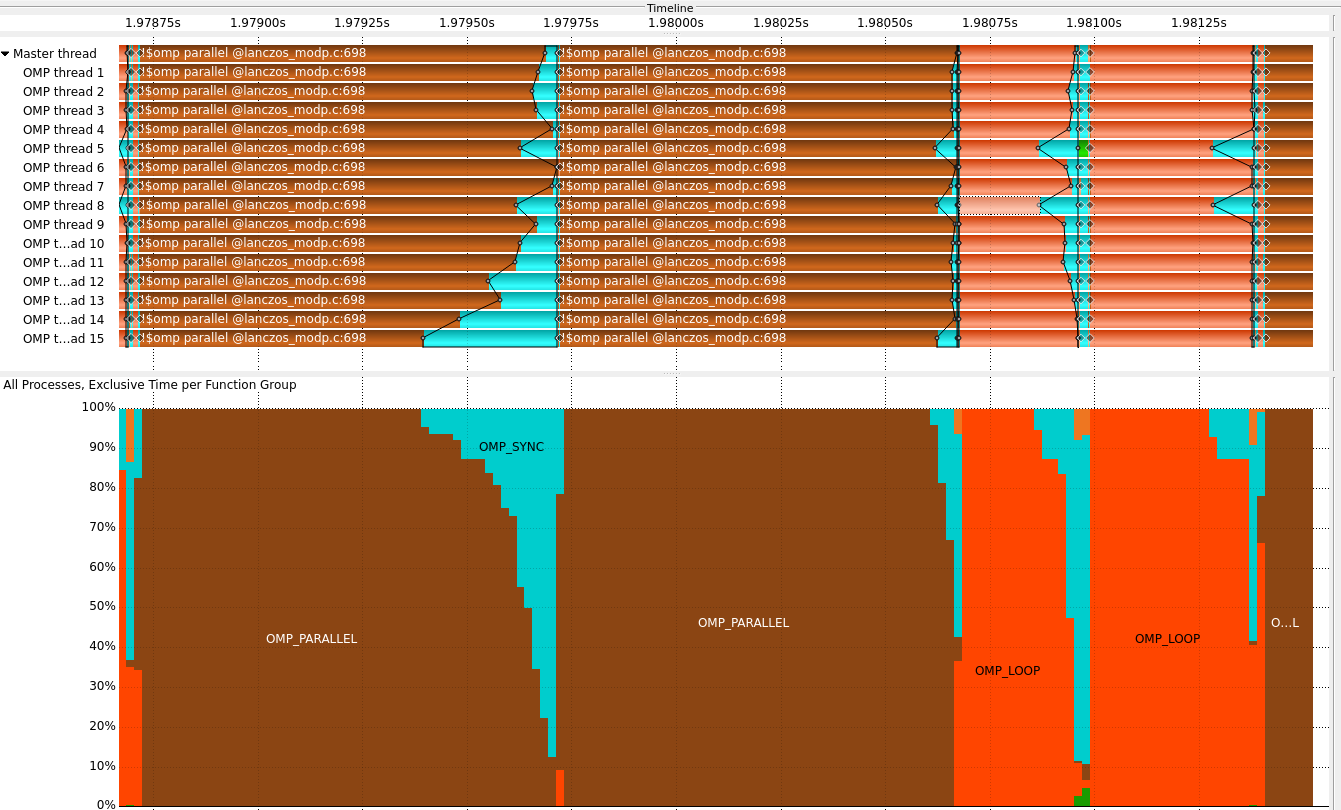
\includegraphics[height=6cm]{vampir.png}
  \end{center}

\begin{block}{Multi-thread}
    \begin{itemize}
    \item Load imbalance (inactive threads)
    \item Time spent waiting for sync. (locks, barriers, ...)
    \end{itemize}
  \end{block}
  
\end{frame}

%%%%%%%%%%%%%%%%%%%%%%%%%%%%%%%%%%%%%%%%%%%%%%%%%%%%%%%%%%%

\begin{frame}
  \frametitle{Traces}

  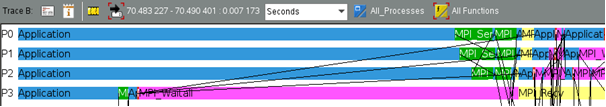
\includegraphics[width=\textwidth]{trace_mpi.png}

  \begin{block}{MPI}
    \begin{itemize}
    \item Time spent in communications
    \item What process delays the others?
    \end{itemize}
  \end{block}  
\end{frame}

%%%%%%%%%%%%%%%%%%%%%%%%%%%%%%%%%%%%%%%%%%%%%%%%%%%%%%%%%%%%

\begin{frame}
  \frametitle{Traces}

  
  \begin{exampleblock}{Advantages}
    \begin{itemize}
    \item Very precise information about dynamic code behavior
    \item Can be obtained automatically (e.g. \texttt{score-p} instrumenter)
    \end{itemize}
  \end{exampleblock}

  
  \begin{alertblock}{Problems}
    \begin{itemize}
    \item Visualization tools are mostly commercial (\texttt{Vampir}, \texttt{itac})
    \item Traces can be \textbf{large} with many processes/threads
    \end{itemize}
  \end{alertblock}
  
\end{frame}

%%%%%%%%%%%%%%%%%%%%%%%%%%%%%%%%%%%%%%%%%%%%%%%%%%%%%%%%%%%%


\end{document}

PAPI

score-p

%%% Local Variables:
%%% TeX-command-extra-options: "-shell-escape"
%%% TeX-engine: luatex
%%% End: